% !TEX root = ../prj4projektrapport.tex
% SKAL STÅ I TOPPEN AF ALLE FILER FOR AT MASTER-filen KOMPILERES 

Til gennemførelse af dette projekt er ASE-modellen blevet anvendt som udgangspunkt. Denne model viser de forskellige faser, projektgruppen skal igennem på vejen mod et endeligt produkt og en veldokumenteret og gennemarbejdet rapport. ASE-modellen ses på figur \ref{fig:Asemodel} Gruppen har desuden anvendt en iterativ og empirisk arbejdsmetode. Der er brugt faglitteratur og teori fra undervisningen til at danne vidensgrundlag for projektet om spændingsregulatoren. Undervejs er der indsamlet nye erfaringer i forbindelse med udviklingen af produktet. 
I udviklingsfasen er der anvendt SysML og UML, der sammen med Use Casene har givet overblik over systemet både grafisk og skriftligt. Dette har dannet grundlag for opbygningen af systemet. 

\begin{figure}[H] 
	\centering
	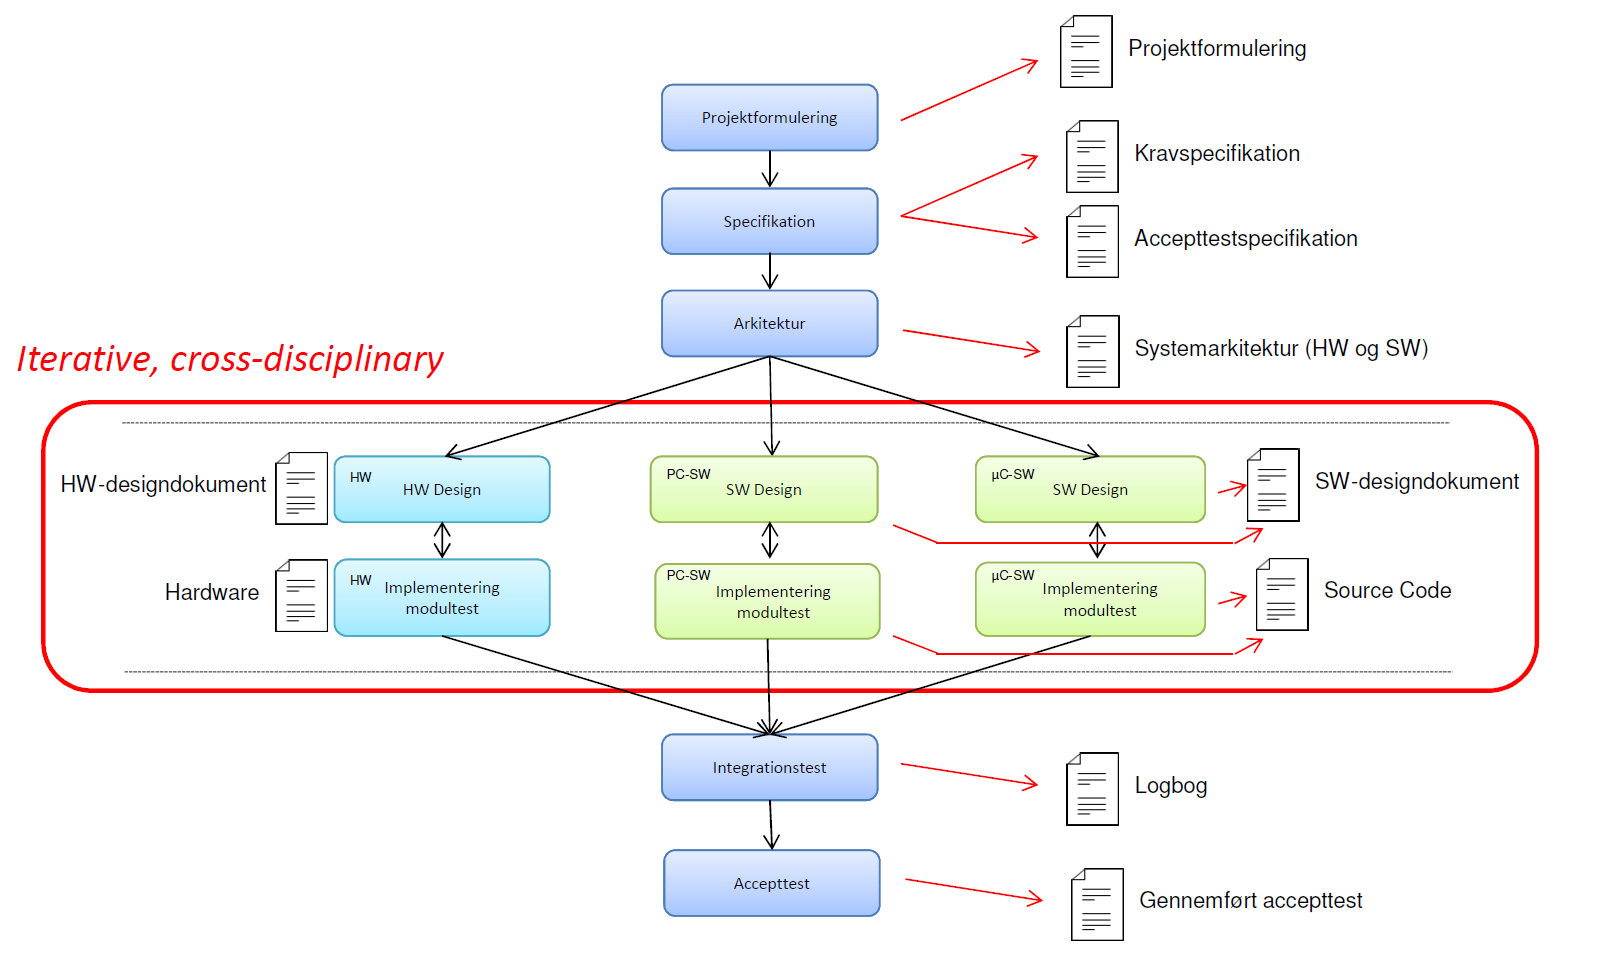
\includegraphics[width=0.7\textwidth]{figure/Asemodel}
	\caption{ASE-modellen}
	\label{fig:Asemodel}
\end{figure}

For at styre og lede projektet har gruppen ladet sig inspirere af Scrum principperne. Fra starten af projektet har gruppen oprettet sprints og defineret dertilhørende opgaver. Gruppen har ikke afholdt daily scrums, men har gennemsnitligt haft 1-2 ugentlige gruppemøder, samt ugentligt vejledermøde. Gruppen udarbejdede desuden en tidsplan for udvikling og rapportskrivning, se bilag. Dette har medført en jævn arbejdsgang og et godt flow i projektet. \newline

Efter udfærdigelsen af arkitekturen for Spændingsregulatoren afholdt gruppen review med en anden projektgruppe. Efter rettelser herfra blev gruppen inddelt i tre hold med hvert sit ansvarsområde. Gennem design og implementeringsfasen har hvert hold haft ansvar for eget arbejdsområde, men den resterede del af gruppen er løbende blevet opdateret i forhold til udfordringer og løsninger. 
Ved integrationstest og accepttest er gruppen igen samlet, og disse udføres i fællesskab. 
Holdinddelingen og ansvarsområder ses i Tabel \ref{tab:arbejdsfordeling}.

% Please add the following required packages to your document preamble:
% \usepackage{booktabs}
% \usepackage{multirow}
\begin{table}[H]
	\centering
	\caption{Arbejdsfordeling}
	\label{tab:arbejdsfordeling}
	\begin{tabular}{@{}lll@{}}
		\toprule
		Holdnr.            & Navn                    & Arbejdsområde                                                  \\ \midrule
		\multirow{2}{*}{1} & Jeppe Hansen            & \multirow{2}{*}{Måleenhed}                                     \\
		& Søren Jensen            &                                                                \\\midrule
		\multirow{2}{*}{2} & Laurids Jørgensen       & \multirow{2}{*}{Styringsenhed}                                 \\
		& Denise Sloth            &                                                                \\\midrule
		\multirow{2}{*}{3} & Caroline Møller Sørensen         & \multirow{2}{*}{Distributionslinje, belastning og Trinskifter} \\
		& Sophia Amalie Mortensen &                                                                \\ \midrule
	\end{tabular}
\end{table}

